\section{Конструкторский раздел}
В данном разделе... (ДОПИСАТЬ)

\subsection{Требования к программному обеспечению}
Требуется реализовать загружаемый модуль ядра для мониторинга приоритетов, времени выполнения и простоя процессов, который будет получать информацию о процессах в режиме ядра и предоставлять доступ к данной информации через procfs.

В целях упрощения работы с данным модулем также потребуется реализовать дополнительную программу, выполняющую загрузку модуля в систему, а также предоставляющую получаемую из procfs информацию без дополнительных манипуляций пользователя.

\subsection{Модуль логирования процессов реального времени}
Для хранения информации о приоритетах, времени выполнения и простоя процессов реального времени выделяется массив символов.

\begin{code}
	\captionof{listing}{Массив символов журнала.}
	\label{code:charLog}
	\inputminted
	[
	frame=single,
	framerule=0.5pt,
	framesep=20pt,
	fontsize=\small,
	tabsize=4,
	linenos,
	numbersep=5pt,
	xleftmargin=10pt,
	firstline=24,
	lastline=25,
	breaklines=true
	]
	{text}
	{../../src/md.c}
\end{code}

Для того, чтобы не допускать переполнений при записи в журнал, каждый раз перед занесением данных в лог проверяется, может ли он в данный момент вместить новые данные.

\begin{code}
	\captionof{listing}{Функция проверки переполнения.}
	\label{code:checkOverflowFunction}
	\inputminted
	[
	frame=single,
	framerule=0.5pt,
	framesep=20pt,
	fontsize=\small,
	tabsize=4,
	linenos,
	numbersep=5pt,
	xleftmargin=10pt,
	firstline=27,
	lastline=39,
	breaklines=true
	]
	{text}
	{../../src/md.c}
\end{code}

\begin{code}
	\captionof{listing}{Пример использования функции проверки переполнения.}
	\label{code:checkOverflowFunctionExecution}
	\inputminted
	[
	frame=single,
	framerule=0.5pt,
	framesep=20pt,
	fontsize=\small,
	tabsize=4,
	linenos,
	numbersep=5pt,
	xleftmargin=10pt,
	firstline=52,
	lastline=58,
	breaklines=true
	]
	{text}
	{../../src/md.c}
\end{code}

Как видно из предоставленного листинга \ref{code:checkOverflowFunctionExecution} в случае обнаружения переполнения модуль прекращает свою работу. Данное решение приведено в целях избежания потери информации при проведении длительного мониторинга, который мог бы включать в себя более 20 итераций без получения информации из procfs.

В листинге \ref{code:proc_ops_realization} приведено заполнение структуры proc\_ops. Требуется, чтобы функция yaRead включала в себя вызов функции copy\_to\_user в целях передачи информации из журнала в пространство пользователя.

\begin{code}
	\captionof{listing}{Заполнение структуры proc\_ops.}
	\label{code:proc_ops_realization}
	\inputminted
	[
	frame=single,
	framerule=0.5pt,
	framesep=20pt,
	fontsize=\small,
	tabsize=4,
	linenos,
	numbersep=5pt,
	xleftmargin=10pt,
	%firstline=52,
	%lastline=58,
	breaklines=true
	]
	{text}
	{code/proc_ops_realization.h}
\end{code}

В листинге \ref{code:initExit} предоставлены функции инициализации и завершения работы модуля.

\begin{code}
	\captionof{listing}{Функции инициализации и завершения работы модуля.}
	\label{code:initExit}
	\inputminted
	[
	frame=single,
	framerule=0.5pt,
	framesep=20pt,
	fontsize=\small,
	tabsize=4,
	linenos,
	numbersep=5pt,
	xleftmargin=10pt,
	firstline=133,
	lastline=154,
	breaklines=true
	]
	{text}
	{../../src/md.c}
\end{code}

В данном фрагменте можно увидеть, что в функции инициализации модуля требуется запустить отдельный поток для журналирования, так как в ином случае инициализация не будет завершена до окончания выполнения требующегося количества итераций сбора информации.

\subsection{Модуль логирования процессов реального времени}

\subsection{Схемы работы модуля и дополнительного программного обеспечения}
На рисунках \ref{fig:useCase}--\ref{fig:useCaseRepo} предоставлены примеры картинок.

\begin{figure}[H]
	\centering
	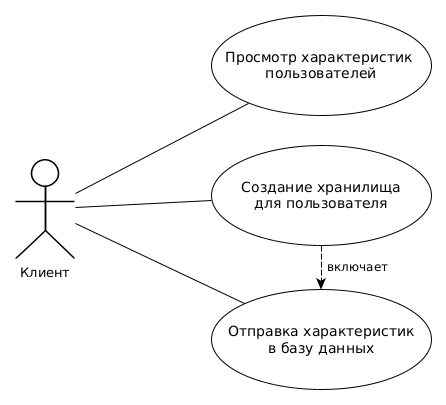
\includegraphics[scale=0.5]{img/useCase.png}
	\caption{Какой-то пример. }
	\label{fig:useCase}
\end{figure}

\begin{figure}[H]
	\centering
	\includegraphics[scale=0.5]{img/useCaseServer.png}
	\caption{Вторая часть какого-то примера. }
	\label{fig:useCaseRepo}
\end{figure}

\subsubsection*{Вывод}
В разделе...

\pagebreak